\section{Introduction}
\label{sec:intro}

Cyber-Physical and IoT Systems such as smart homes, industrial control and healthcare systems often require the correct functioning of a myriad set of sensors. 
%IoT applications deployed in smart homes, industrial control and healthcare systems require the correct functioning of a myriad set of sensors. 
%
%The sensors allow such systems to measure their environment and, trigger computations and actions. 
% that are part of their intended design.
%
These sensors measure the surrounding environment in the form of either an arithmetic value (\eg temperature of 72\degree F) or a logical value (\eg presence or absence of smoke) and, trigger computations and actions.
% 
Typically, these sensor data measurements are used by data-driven IoT analytics pipelines (\eg Microsoft Azure IoT) to derive insights and make higher-level decisions. 
%The data from these sensors is used by IoT analytics pipelines to derive patterns, insights and make decisions.
%
%In this paper, we will be looking at a Passive Infra-Red (PIR) sensor.
%
One of the most versatile and ubiquitous sensors used in numerous modern applications is a Passive Infra-Red (PIR) sensor.
%
A PIR sensor is a discrete, electronic sensor that captures thermal radiation from human and human-like objects (\eg animals) to indicate occupancy in a region. %its field of view.
%
They are used in a wide-variety of environments -- \eg in offices to achieve energy savings in buildings (for automatic control of lighting and HVAC systems) and in safety-critical cyber-physical systems (CPS) like factory floors for intrusion detection.
%They are used in a wide variety of environments, from building automation to safety-critical systems such as factories. 
%{\bfseries Fig.~\ref{fig:pir_in_smart_building}} shows PIR sensors in a modern building, where it is used to achieve energy and operational cost savings~\cite{PricewaterhouseCoopers}. 
%
%Consequently, the correct operation of PIR sensors is critical to the quality and performance of many IoT deployments.
Naturally, these applications mandate the correctness and fidelity of data \ie the data being a faithful representation of occupancy.
%and trigger computations or actions as per application requirements.}
%
%\ashish{what generic class of sensor?characteristics functionality. applications, general problems. go to failures.lets look at pir. then go into pir}
%
%An example of using occupancy sensor in smart buildings is shown in {\bfseries  
%  \eg automatic control of lighting and HVAC systems) 
%to even safety-critical systems such as manufacturing systems. 
% \subsection{Motivation}

%Unfortunately, these sensors are prone to failures and degradation of physical components. 
%
Given the nature of PIR deployments in the wild : for instance in remote, manually inaccessible, harsh conditions (\eg assembly line of a factory), they are prone to failures and degradation of physical components.
%
% In the case of the PIR\footnote{We focus on PIR in this paper though our observations are broadly applicable.} 
%
% In the case of the PIR sensor, 
% These failures could result in false triggers or failure to capture real movements \eg conference room lights turning off or doors not opening in spite of occupancy . 
%
These failures could result in false triggers or a failure to capture real movements \eg assembly line failures in a factory, inaccurate estimation of wildlife counts, conference room lights turning off or even doors not opening in spite of occupancy.
%
Such sensor failures are often caused by intermittent sensor faults that can happen in any one of its internal physical components~\cite{chakraborty2018fall,marathe2021currentsense}.
%
% shown in {\bfseries Fig. \ref{fig:pir_system_teardown}}, ~\eg physical damage to the lens or condensation damage to the optical filter. 


%A passive infrared sensor (PIR sensor) is a discrete, electronic sensor that captures thermal radiation from human and human-like objects (\eg animals) to indicate the occupancy in its field of view. The output of PIR sensor is in the binary form, indicating \textit{the presence (or absence)} of an object\footnote{We use the terms obstacle, object and human object interchangeably in this paper}. They are used in a wide-variety of environments -- \eg in offices to achieve energy savings in buildings (for automatic control of lighting and HVAC systems) and in safety-critical cyber-physical systems (CPS) like factory floors for intrusion detection. Naturally, these applications mandate the correctness and fidelity of data \ie the data being a faithful representation of the presence (or absence) of an object.



%Despite surging in usage, it remains an unfortunate fact that PIR sensors are prone to false triggers as well as missing presence of objects. For example, it sometimes happens that lights in conference rooms to accidentally turn off despite motions and fail to turn on unless one waves their arms around aggressively for the sensors to capture motion. Phenomena such as these are caused mostly due to intermittent sensor faults. A system teardown of the PIR sensor is shown in Fig.~\ref{fig:pir_system_teardown} and faults can happen in any of these components~\eg physical damage to the lens or condensation damage to the optical filter.

% \begin{figure}[htbp] 
	% 	%%%%%%%%%%%%%%%%
	% 	% SMART BUILDING
	% 	%%%%%%%%%%%%%%%%
	% 	\begin{minipage}[t]{0.5\textwidth}
		% 		%\begin{figure}
		% 		\centering
		% 		%\begin{flushleft}
		% 		%\includegraphics[width=1.0\columnwidth]{figures/platform/pir-sensor-internals-combine-with-3d.png}
		% 		\includegraphics[width=0.8\textwidth]{figures/motivation/PIR-applications-in-smart-buildings.png}
		% 		%\end{flushleft}
		% 		\caption{\textbf{Applications of PIR sensor} in Smart Buildings.}
		% 		%\vspace*{-0.5\baselineskip}
		% 		\label{fig:pir_in_smart_building}
		% 		%\end{figure}
		% 	\end{minipage}%
	% 	%%%%%%%%%%%%%%%%
	% 	% END OF SMART BUILDING
	% 	%%%%%%%%%%%%%%%%
	% \end{figure}

%\begin{figure}
%%%%%%%%%%%%%%%%
% MOTIVATION FOR PHYSICS
%%%%%%%%%%%%%%%%
\begin{wrapfigure}{R}{0.5\textwidth}
	\centering
	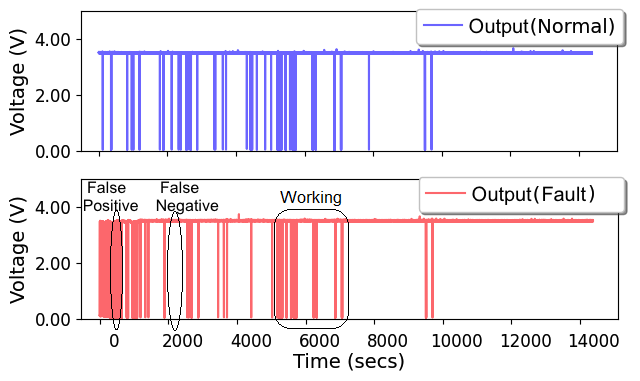
\includegraphics[width=0.5\textwidth]{figures/motivation/motivation-physics-technique.png}
	\caption{\footnotesize{Sensor Data} from a working PIR (top) and a faulty PIR (bottom). HIGH indicates no object, HIGH$\rightarrow$LOW transition indicates object.}
	\label{fig:occupancy_sensor_data}
\end{wrapfigure}
%%%%%%%%%%%%%%%%
% END MOTIVATION FOR PHYSICS
%%%%%%%%%%%%%%%%

% \begin{figure*}%[htbp]
	% 	%%%%%%%%%%%%%%%%
	% 	% SENSOR TEARDOWN
	% 	%%%%%%%%%%%%%%%%
	% 	\begin{minipage}[b]{0.25\textwidth}
		% 		\begin{flushleft}
			% 		%\begin{figure}
			% 		%\centering
			% 		%\includegraphics[width=1.0\columnwidth]{figures/platform/pir-sensor-internals-combine-with-3d.png}
			% 		%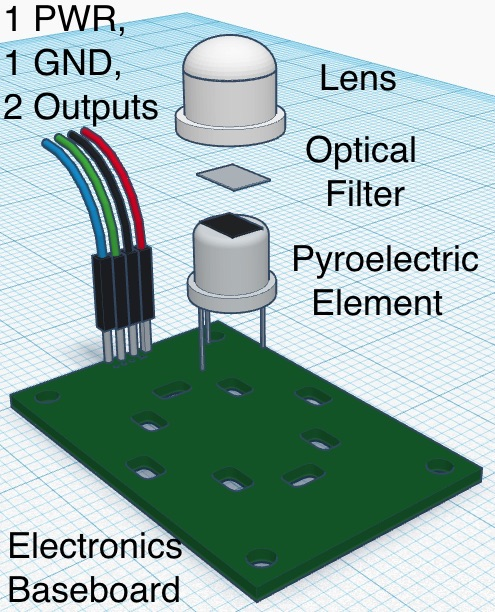
\includegraphics[height=1.5in]{figures/platform/3d_view_5-annotated.jpg}
			% 		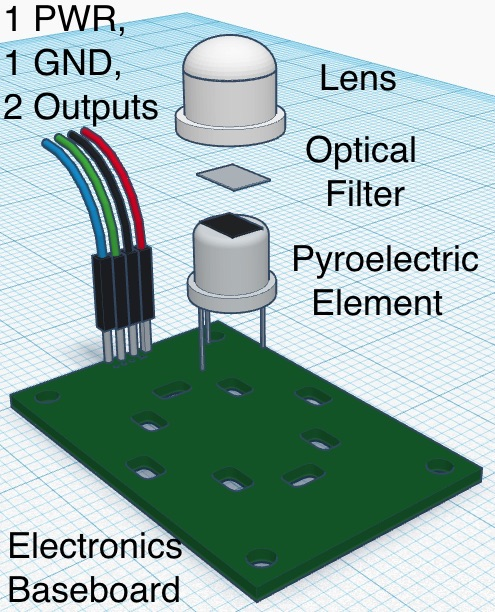
\includegraphics[width=0.9\textwidth]{figures/platform/3d_view_5-annotated.jpg}
			% 		\end{flushleft}
		% 		\caption{\textbf{PIR Sensor Teardown}}
		% 		%\vspace*{-0.5\baselineskip}
		% 		\label{fig:pir_system_teardown}
		% 		%\end{figure}
		% 	\end{minipage}%
	% 	%%%%%%%%%%%%%%%%
	% 	% END OF SENSOR TEARDOWN
	% 	%%%%%%%%%%%%%%%%
	% 	\hspace{5ex}
	% 	%%%%%%%%%%%%%%%%
	% 	% PIR SENSOR PIPELINE
	% 	%%%%%%%%%%%%%%%%
	% 	%\begin{subfigure}{0.48\textwidth}
	% 	\begin{minipage}[b]{0.60\linewidth}
		% 		%\begin{flushright}
		% 		\centering
		% 			\begin{subfigure}[t]{\textwidth}
			% 				\includegraphics[width=\textwidth,height=0.9in]{figures/platform/pir-block-diagram-2.png}
			% 				\caption{}
			% 				\label{fig:pir_sensor_pipeline}
			% 			\end{subfigure}\\
		% 			\begin{subfigure}[t]{\textwidth}
			% 				\includegraphics[width=\textwidth,height=0.7in]{figures/platform/sensys_workflow.png}
			% 				\caption{}
			% 				\label{fig:system_workflow}
			% 			\end{subfigure}
		% 		%\end{flushright}
		% 		\caption{\ca \textbf{Physics of the} PIR Sensing Pipeline, \cb \textbf{End-to-end workflow} of \sol for fault detection and diagnosis.}
		% 		\label{fig:pir_sensing_pipeline}
		% 	\end{minipage}
	% 	%\end{subfigure}%
	% 	%%%%%%%%%%%%%%%%
	% 	% END OF PIR SENSOR PIPELINE
	% 	%%%%%%%%%%%%%%%%
	% \end{figure*}    


%\begin{figure}[t]
%	\centering
%	\small
%	\begin{subfigure}[t]{0.5\textwidth}
	%		\centering
	%		\includegraphics[width=\textwidth]{figures/platform/pir-block-diagram-2.png}
	%		\caption{\textbf{PIR Sensing Pipeline} showing the physics.}
	%		\label{fig:pir_sensor_pipeline}
	%	\end{subfigure}\\
%	\begin{subfigure}[t]{0.5\textwidth}
	%		\centering
	%		\includegraphics[width=\textwidth]{figures/platform/sensys_workflow.png}
	%		\caption{\textbf{End-to-end Workflow} for performing data capture and fault analysis of PIR sensors.}
	%		\label{fig:system_workflow}
	%	\end{subfigure}
%\end{figure}

Currently, failures in PIR sensor deployments are usually addressed in one of the following two ways : \ca using an additional, auxiliary sensor such as a CCTV camera combined with image processing algorithms (say to validate the occupancy data) or \cb using high-grade PIR sensors that possesses additional capabilities such as ultrasonic sensors and intricate optics. This makes the sensor deployment very expensive. % with intricate optics and added capability such as ultrasonic sensors. 
In addition, deployments need to be refreshed periodically by replacing old sensors with new ones and the former are disposed off %trashed 
adding to both electronic waste and cost. A case in point is our university research building where the occupancy sensor deployed is a high-grade PIR sensor comprising both ultrasonic and infrared sensors, resulting in a \emph{total recurring cost of close to \$100000 every 10 years}\footnote{Our 4-floor building (with a total of 244 rooms and 24 aisle areas) has more than 300 occupancy sensors. Each PIR sensor costs \$300~\cite{hubbell_ADT1600WRP, hubbell_ATD2000CRP} with it being refreshed every 10 years, a worst-case recurring cost of \$90000 every 10 years, which is expensive.}.


\begin{comment}
	%%%%%%%%%%%%%%%%
	% MOTIVATION FOR PHYSICS
	%%%%%%%%%%%%%%%%
	\begin{wrapfigure}{L}{6cm}
		\centering
		\vspace{-10pt}
		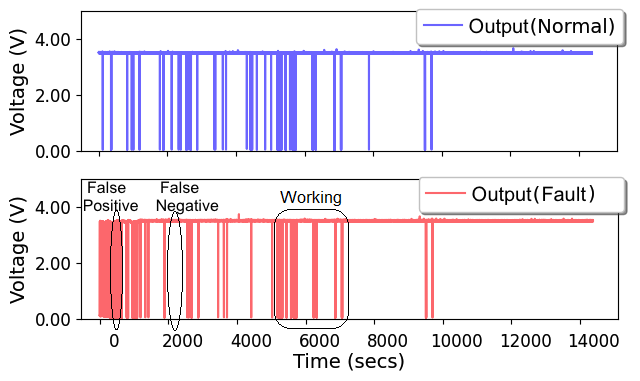
\includegraphics[width=0.4\columnwidth]{figures/motivation/motivation-physics-technique.png}
		\caption{\textbf{Occupancy Sensor Data} from a working sensor (top) and a degraded sensor with some dust deposited on the lens (bottom). The output follows negative logic \viz 0 -- object, 1 -- no object.}
		%\vspace*{-1.0\baselineskip}
		\label{fig:motivation_physics}
		\vspace{-10pt}
	\end{wrapfigure}
	%%%%%%%%%%%%%%%%
	% END MOTIVATION FOR PHYSICS
	%%%%%%%%%%%%%%%%
\end{comment}

Crucially, \textit{current approaches do not diagnose the cause of failures or perform any analysis of sensor performance}, that can be valuable for IoT %smart building 
engineers during maintenance, repair and testing. For example, in one of our deployments, we observed that failed or degraded sensors can exhibit unpredictable behavior \eg they can work temporarily for a period of time and then fail sometimes. {\bfseries  Fig.~\ref{fig:occupancy_sensor_data}} shows a plot of output data from the sensor vs. time for both a working sensor and a faulty sensor (defective lens) over a period of 4 hours.
% \footnote{Internals of PIR sensor are covered in \S\ref{sec:approach}}. 
In this plot, a transition from HIGH$\rightarrow$LOW denotes a person coming into the field of view %an obstacle 
and a value of HIGH indicates that there is no person. %obstacle.
We observe that the faulty sensor works intermittently and at other times, can miss a person (false negative) or incorrectly flag the presence of a person (false positive).
%In {\bfseries  Fig.~\ref{fig:occupancy_sensor_data}}, we see that the faulty sensor missed a person %n obstacle 
%
%around 6:45 pm, whereas the same faulty sensor worked correctly through 6 pm. These failures can evade failure detection schemes that are purely data-driven since the data looks good up to 6:45 pm.
%
Missing a person can cause a potentially critical failure in applications such as door opening systems or emergency shutdowns on factory floors.
%
We show that accurate detection of such failures is possible by \textit{characterizing the internals of the sensor.}
%
%Additionally, physics-based reliability techniques can be used to augment AI/ML-based cloud IoT analytics pipelines.% 
%
%\eg Microsoft Azure IoT.
%In addition, extra sensors also require extra power using power packs such as CU-300A~\cite{hubbell_power_pack_cu300a} that only add to the cost.
%While both these approaches partially offset the issue albeit at a high cost, from an engineering standpoint, it makes the reliability of the composite system to be dependent on the additional sensor (\eg camera) as well that of the PIR sensors -- thereby reducing the failure probability. 

% In a nutshell, current solutions to faulty/incorrect sensor data \ca make the deployment expensive (additional auxiliary or high-grade sensors), \cb add to potential electronic waste (sensors are refreshed periodically) and \cc they do not diagnose failures. Thus, we need to look for alternative approaches.

\begin{comment}
	\begin{tcolorbox}%[top=0.05pt,bottom=0.05pt,boxsep=0pt,toptitle=0.1ex,bottomtitle=0.1ex]
		[left=0.05pt,right=0.05pt,top=0.05pt,bottom=0.05pt,boxsep=0pt,toptitle=0ex,bottomtitle=0ex,sharp corners]
		{\bfseries Summary:} Existing solutions for reliability in IoT sensors: \ci require additional, auxiliary sensors, \cii do not diagnose failures, and \ciii add to electronic waste, resulting in large recurring cost.
	\end{tcolorbox}
\end{comment}
% \subsection{Our Study and Results}

\emph{Our solution, \sol detects and diagnoses failures of PIR sensors by characterizing the physics of sensing} \viz the fresnel lens optics and the pyroelectric effect. % and analyzing the various subsystems in action through the sensing pipeline. 
%
To keep the cost of the deployment low, \sol is implemented on the edge platforms of the deployment and targets commodity PIR sensors.
%
In this process, %the process of characterizing the physics, 
we \emph{devised a taxonomy of key failures for aiding diagnosis and repair.} 
%This does not require any additional auxiliary sensor and can thus be used to develop low-cost solutions to validate the correctness and fidelity of sensor data.

Specifically, we demonstrate that a signal intrinsic to PIR sensors~\viz the \textit{intermediate analog output from the pyroelectric element, referred to as \aout} ({\bfseries Fig.~\ref{fig:pir_sensing_pipeline}}) can be used for %has 
fault detection and diagnosis. % capabilities. % and performance monitoring capabilities. 
%
We utilize this signal to derive information about reliability of the PIR sensor platform as well as to perform an analysis into the different failure modalities. \textit{To the best of our knowledge, this is the first edge-based, low-cost approach to use an intrinsic signal (\aout) for fault detection and diagnosis of PIR sensors.} We analyze the behavior of \aout in detail, under %various conditions -- both in a controlled setting in the lab as well as in
practical deployments, with realistic occupancy
%(both before and during pandemic~\cite{doi:10.1056/NEJMe2002387})
over a wide variety of observed failures. 
%Note that we do not use any auxiliary or high-grade sensor and thus this approach can be used to develop low-cost solutions to validate the correctness and fidelity of sensor data.

\noindent \textbf{Summary of Contributions:}
%\vspace{-5pt}
\begin{enumerate}[leftmargin=*]
	\itemsep0pt
	\item \textit{From physics to failures:} We use the working of a PIR sensor to understand the process of object detection and infer the key points where failures could lead to incorrect sensor data,
	\item \textit{Failure taxonomy:} We study the impact of different failures on the sensor performance and systematize the key failures into a failure taxonomy. We also provide a quantitative method to study the severity of failures.
	% Note that while the taxonomy is PIR-specific, the core principles can be applied to other sensors as well.
	% and analyze the performance under different failure scenarios.
	
	\item \textit{Non-intrusive, online fault detection and diagnosis:} We present an online technique (does not require any disassembling), \emph{implemented at the edge}, for failure detection as well as diagnosis by utilizing the intermediate, analog output from the pyroelectric element in the PIR sensor (\aout). 
	%
	%The technique is completely online (does not require any disassembling) and is implemented at the edge device. 
	%
	%We demonstrate the use of \aout as a proxy to classify between faulty and working sensors.
	%
	%In addition to classification, we also show how \aout can be used to diagnose the failures \ie failure identification.
	%
	% ({\bfseries Fig.~\ref{fig:system_workflow}})
	\item \textit{Insights from Real-world Deployments:} We show the efficacy of the proposed techniques using a deployment of 15 PIR sensors in four practical occupancy scenarios over a period of 3 months.
	%(elevator, lobby of a building and at starbucks)
	% across two countries
	%(India, US)
	% -- both before and during the SARS-CoV-2 (Covid-19) pandemic~\cite{doi:10.1056/NEJMe2002387}. 
	% We use our techniques to detect and analyze faults occurring in practice.
\end{enumerate}

% \textbf{Impact:} Due to lack of standard designs of PIR sensors, we propose all the sensor vendors to include the \aout signal in all PIR sensor design standards to aid in the reliability of PIR sensors. This enables low-cost edge-based fault detection and diagnosis.% to be implemented at the Edge at low cost and minimal electronic waste.
% \ashish{say that its not real-time but it is online and computing is on the edge and not on backend clouds.}

\begin{comment}
	\subsection{Assumptions}
	\quad \underline{\bfseries Target System:} We consider PIR sensor deployments that are: \ca large in scale, \cb deployed remotely (making manual checking of faults hard), \cc consisting of low cost and \cd commodity off the shelf (COTS) sensors, such as those in modern smart buildings.
	%in that comprise of a large number of low-cost sensors that can degrade or fail. 
	%\ins{Being low-cost, these sensors have low compute or storage capabilities.}
	
	\underline{\bfseries Choice of sensor:} As our work leverages the \aout signal present in a PIR sensor, we require a PIR sensor that allows access to \aout either directly or indirectly by reworking the sensor such as ~\cite{PIR_sensor_eval}. While this limits the scope of our work, our framework can form the basis for manufacturers and IoT engineers for leveraging the rich information in \aout for inclusion in future designs.
	%Commercial occupancy sensors are of 4 different types of technologies : \ci Microwave antenna-based, \cii Ultrasonic-based, \cii Passive Infra-Red (PIR) or \civ Photocell (PC) based. Among these four technologies, PIR is the most commonly used, the cheapest, available from the largest number of vendors and also used in our buildings both in India and in the US. Thus, we chose PIR-based occupancy sensors for our analysis.
	
	\underline{\bfseries Existence of ground truth:} We perform our analysis of the occupancy patterns by gathering data from multiple different sensors, some of which can fail or degrade. However, we assume that not all sensors fail simultaneously as it enables us to separate physics of failed sensors from physics of working sensors. This is a reasonable assumption due to the large-scale nature of deployment.
	
	\underline{\bfseries Security of sensor values:} We perform our analysis of sensors at the edge, and assume that the sensor data are not tampered with using attacks such as Man-in-the-Middle attacks (MitM) or using software vulnerabilities in the edge platform.
\end{comment}

\noindent \textbf{Goals:}

\begin{enumerate}[leftmargin=*]
	\itemsep0pt
	
	\item {\itshape Detect failures:} Sensors can give faulty data due to the incorrect operation of various physical components involved in the sensing process. We seek to detect and isolate such failed sensors. %data that is not a faithful representation of the physical phenomenon.
	%
	
	\item {\itshape Diagnose failures:} In addition to detecting failures, we perform failure diagnosis to identify the cause of the failure. We use domain-knowledge of the sensing physics and our understanding of how different failures can impact the physics. This aids in repair and performing quality-control checks.
	%
	
	\item {\itshape Edge-based solution:} \sol is tailored for edge platforms (Raspberry Pi, Arduino Microcontrollers) that are interfaced directly to multiple sensors, say via GPIO. %\st{Being low-cost, these sensors have low compute or storage capabilities.}
	Edge-based reliability solutions allows us to reject data from faulty sensors in IoT deployments thus saving the cost of both \ca the edge to cloud network bandwidth and \cb cloud compute consumed by faulty data.
	%
	
	\item {\itshape Target Audience:} \sol benefits two sections of the community: \ca engineers developing and deploying IoT/Edge computing for occupancy sensors (\eg Smart Buildings), \cb manufacturers of occupancy sensors can use the insights from this work towards future PIR sensor hardware designs.
	
	%We first present the background, physics of the PIR sensor and our failure taxonomy. Next, we present details about the intrinsic hardware signal and analyse its behavior under the failure scenarios. Thereafter, we deploy our sensors in the wild for evaluation and conclude with lessons learnt from the real-world failures.
\end{enumerate}

\begin{comment}
	Sensors are the bridge between the compute domain and the physical domain. They provide a manifestation of the physical domain to the compute domain wherein the computation is then be performed. The result of this computation is then utilized to make changes to the physical domain. For example, when a user moves his palm under a faucet with an in-built sensor, it triggers a signal to open a valve that pours water onto his palms. This closed loop of $physical\_environment \rightarrow sensor \rightarrow compute \rightarrow actuator \rightarrow physical\_environment$, seen in all sensing systems excludes reliability measures such as failure detection and sensor drift. As a result, we currently piggyback techniques such as data-driven anomaly detection \cite{hill2010anomaly} and schemes as calibration \cite{maag2018survey} to existing systems to achieve reliability and confidence in the data.  Additionally, present techniques for hardware fingerprinting apply to a restricted class of sensors - analog sensors, which operate by periodically sampling a quantity of interest and where the voltage variation between the on and off states are high enough to be characterized. 
	
	% In this work, we integrate failure detection as a first class citizen in the sensing process by expressing it as a function hardware characteristics of the sensor. 
	
	In this paper, we present an automated, low-cost approach to fault detection in digital sensors, performed at the edge, without user intervention. We perform this by analyzing sensors which are outside the purview of the \textit{Fall-curve} \cite{chakraborty2018fall} technique. As sensors vary in nature by the phenomena being sensed, leading to different physics of operation, and hardware signals, there is no single silver bullet to detect faults. Instead, we present a suite of techniques based on most commonly found faults in the wild. %For example, different sensors use different physical principles to sense different kinds of physical variables such as temperature, pressure, and humidity among others. Additionally, due to the varying underlying principles, they also have different electronic and/or mechanical components.
	
	
	\newenvironment{myquotation}{\setlength{\leftmargini}{1.5em}\quotation}{\endquotation}
	\begin{myquotation}
		\noindent\textit{We present a principled approach to making digital sensors "reliable" - overcoming the challenges of capturing fall curve \cite{chakraborty2018fall} and finding alternative approaches to capture the hardware fingerprint of the sensor.}
	\end{myquotation}
	
	\noindent \textbf{Scope} We consider digital sensors out there are low cost, used in large scale, and are deployed in remote and harsh environments. From an application standpoint, we looked at sensors that are used in environmental monitoring.
	
	
	% \noindent \textbf{Our Approach}  Our approach entails using a \textit{systems} approach and thus requires us to understand the different systemic signals present in such sensors. We emphasize that these signals are disparate from the data that is being measured, making it independent of the environment and unique for a type of sensor. Examples of such signals include warm-up behavior, current consumption of different components during the sensing process, voltages at various intermediate points in the sensor circuitry before, during and after sensing and so on. In turn, identifying such signals requires us to understand the different components present in the sensor. It is to be noted that we need not understand every single electronic component in the sensor going all the way down to discrete circuit components as such an approach is neither scalable nor feasible. Furthermore, with increasing sophistication and reliability of manufacturing technology and the integrity checks in place at the fabrication, failures in the electronics are better handled by the conventional integrated circuit testing practices \cite{weste1985principles}. Instead, we analyze failures on a macro level at the granularity of a \textit{subsystem}. Our focus is on \textit{subsystems} that are prone to fail in the common case as discerned from failure reports and interaction with industry collaborations \cite{}. Broadly, our approach consists of four steps : \ci Studying and understanding physics of functional sensors, \cii Analyzing the different physical blocks present in the sensor, \ciii Identifying points of failure in each of the blocks, and \civ Devising techniques to monitor the blocks for failures.
	
\end{comment}